% Created 2023-07-07 Fri 18:29
% Intended LaTeX compiler: pdflatex
\documentclass[11pt]{article}
\usepackage[utf8]{inputenc}
\usepackage[T1]{fontenc}
\usepackage{graphicx}
\usepackage{longtable}
\usepackage{wrapfig}
\usepackage{rotating}
\usepackage[normalem]{ulem}
\usepackage{amsmath}
\usepackage{amssymb}
\usepackage{capt-of}
\usepackage{hyperref}
\usepackage{listings}
\usepackage{tikz}
\usepackage{xcolor}
\definecolor{identifiercolor}{rgb}{0.36, 0.54, 0.66}
\definecolor{keywordcolor}{rgb}{0.93,0.79,0.69}
\definecolor{commentcolor}{rgb}{0.66,0.66,0.66}
\definecolor{stringcolor}{rgb}{0.75, 0.5, 0.51}
\lstdefinelanguage{nix}{
  % Anything betweeen $ becomes LaTeX math mode
  mathescape=false,
  % Comments may or not include Latex commands
  texcl=false,
  keywords=[1]{inherit,import,if,then,else,false,true,or,rec,let,in,assert,with},
  % Comments delimiters, we do turn this off for the manual
  comment=[l]{\#},
  morecomment=[s]{/*}{*/},
  % Spaces are not displayed as a special character
  showstringspaces=false,
  % String delimiters
  morestring=[b]",
  morestring=[d]'',
  % Size of tabulations
  tabsize=2,
  % Enables ASCII chars 128 to 255
  extendedchars=false,
  % Case sensitivity
  sensitive=true,
  % Automatic breaking of long lines
  breaklines=false,
  % Default style for listings
  basicstyle=\small\ttfamily,
  % Position of captions is bottom
  captionpos=b,
  % flexible columns
  columns=[l]fixed,
  % Style for (listings') identifiers
  identifierstyle={\ttfamily\color{identifiercolor}},
  % Style for declaration keywords
  keywordstyle={\bfseries},
  % Style for strings
  stringstyle={\ttfamily\color{stringcolor}},
  % Style for comments
  commentstyle={\ttfamily\color{commentcolor}},
}[keywords,comments,strings]

\author{Rory Tyler Hayford}
\date{\today}
\title{}
\hypersetup{
 pdfauthor={Rory Tyler Hayford},
 pdftitle={},
 pdfkeywords={},
 pdfsubject={},
 pdfcreator={Emacs 28.2 (Org mode 9.5.5)}, 
 pdflang={English}}
\begin{document}

\setcounter{tocdepth}{3}
\tableofcontents

This is a simplified example of an automated lumberjack configuration process with example Nix code. It illustrates how a user could install and configure the \texttt{single-well-controllogix} driver. The workflow and example code make the following assumptions:
\begin{itemize}
\item The lumberjack to be configured has already been created (and has a serial number)
\item We have a method of reusing existing \texttt{onping-api} (or other OnPing) routes
\item The only driver configuration option for \texttt{single-well-controllogix} corresponds to calling OnPing's \texttt{/control/logix/location/add} route
\begin{itemize}
\item Note that this simplifies the example modules presented, because we do not need to deal with any impure intermediate results
\end{itemize}
\item The Haskell executable (referred to as \texttt{lumberjack-automate}) has been deployed on a server
\end{itemize}

\section*{Diagrams}
\label{sec:orgd2f4682}
\subsection*{Deployment}
\label{sec:org9681d48}
This illustrates a simplified deployment. \texttt{lumberjack-automate} is assumed to be deployed on a server having been configured to interact with the flake (i.e. SSH authentication and binary cache setup):
\begin{center}
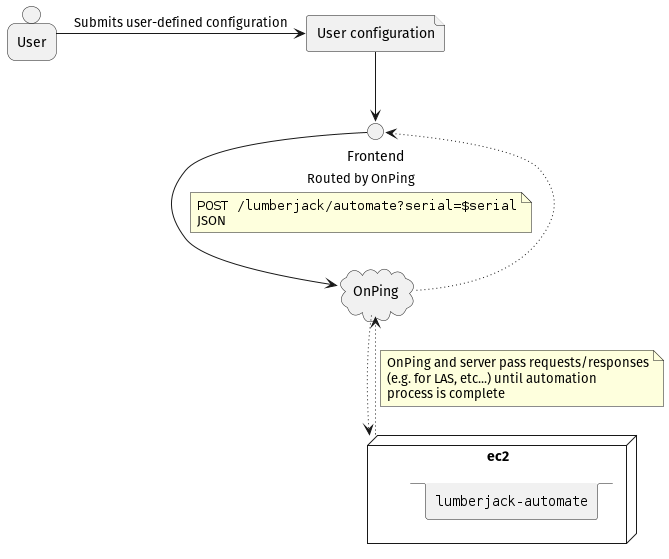
\includegraphics[width=.9\linewidth]{./deploy.png}
\end{center}
The operations of \texttt{lumberjack-automate} are illustrated below.
\subsection*{\texttt{lumberjack-automate}}
\label{sec:org56ea7fc}
This illustrates the processes and interfaces necessary for the driver installation and configuration to occur:
\begin{center}
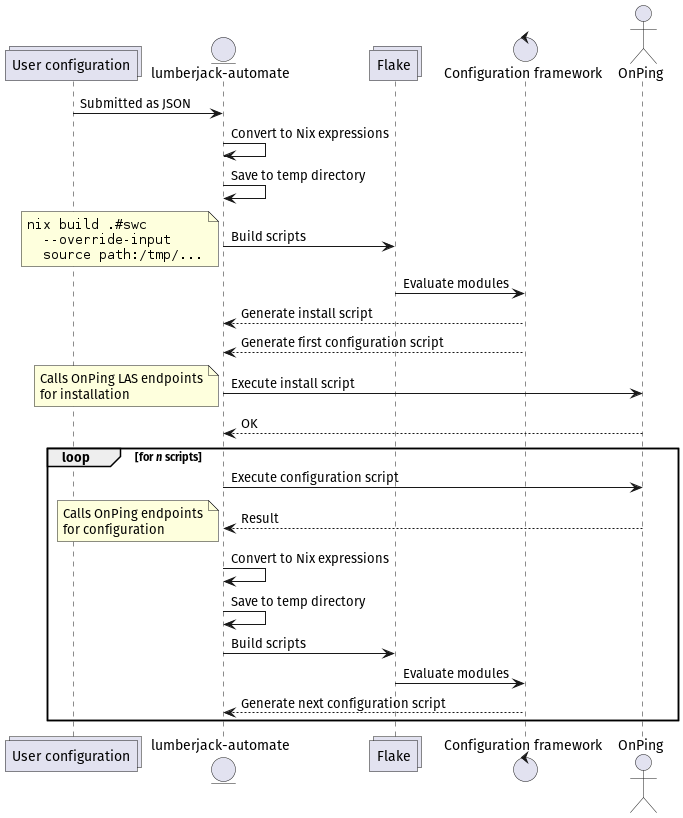
\includegraphics[width=.9\linewidth]{./automate.png}
\end{center}
\section*{Examples}
\label{sec:org43af963}
Note that this example is simplified and assumes that we can generate the installation script and a single configuration script for \texttt{single-well-controllogix} at the same time. This makes the example more concise but in practice, each driver will have several separate modules, which is not illustrated below.
\subsection*{Flake}
\label{sec:orga14523e}
As described in the original outline, the configuration framework would be exposed as applied functions from a dedicated flake. The flake would use an input to parameterize functions that generate the configuration scripts using the Nix module system.
\lstset{language=nix,label= ,caption= ,captionpos=b,numbers=none}
\begin{lstlisting}
{
  inputs = {
    nixpkgs.follows = "all/nixpkgs";
    all.url = "ssh+git://git@github.com:plow-technologies/all";
    # By default, this is an empty Nix expression. It will
    # be overriden by `lumberjack-automate` to evaluate the
    # modules
    source.url = "path:./noop.nix";
    source.flake = false;
  };
  outputs = { self, nixpkgs, all, source, ... }:
    let
      system = "x86_64-linux";
      pkgs = all.legacyPackages.${system};
      # These are functions that evaluate the Nix
      # expression using the modules illustrated
      # below, ultimately generating the configuration
      # scripts
      modules = import ./modules {
        inherit pkgs;
      };
    in
    {
      # We can use `legacyPackages` instead of
      # `packages` in order to nest the several
      # configuration scripts
      legacyPackages = {
        single-well-controllogix =
          modules.single-well-controllogix
            (import source);
        ;
      };
    };
}
\end{lstlisting}
\subsection*{Configuration modules}
\label{sec:orged1917c}
The configuration framework modules would be defined in the same repository as the flake. For this example, a single module is illustrated that would generate an installation script and a configuration script (to add a location) for \texttt{single-well-controllogix}. In reality, each driver will almost certainly have separate modules for generating different configuration scripts.
\lstset{language=nix,label= ,caption= ,captionpos=b,numbers=none}
\begin{lstlisting}
# In modules/single-well-controllogix.nix
let
  cfg = config.drivers.single-well-controllogix;
in
{
  options = {
    enable = lib.mkEnableOption
      (lib.mdDoc "single-well-controllogix");

    configuration = lib.mkOption {
      description = lib.mdDoc "...";
      type = lib.submodule {
        options = {
          name = { /* ... */ };
          plcPort = { /* ... */ };
          pollTimeSeconds = { /* ... */ };
          companyName = { /* ... */ };
          siteId = { /* ... */ };
          groupId = { /* ... */ };
          # Optional
          latitude = { /* ... */ };
          longitude = { /* ... */ };
        };
      };
    };
  };

  config =
    let
      # We can also use common options for all modules
      inherit (config.onping)
        url port;

      conf = builtins.toJSON
        (
          cfg.configuration // {
            # This would also be a common option
            lumberjackID = config.lumberjack.id;
          }
        );
      # We can use the package set from `all` to create the package set
      # to install. This could also be a single installation script for
      # all of the modules (instead of per driver). This is one reason
      # that the flake needs to interface directly with `all` (so we
      # know which Nix paths each package corresponds to, etc...)
      packages = utils.mkPackageSet { /**/ };
    in
    lib.mkIf cfg.enable {
      scripts = {
        install = pkgs.writeShellApplication {
          name = "install-swc";
          runtimeInputs = [ pkgs.curl ];
          text = ''
            curl -X POST \\
             ${url}:${toString port}/lumberjack/deploy/package/install \\
              -d '${packages}'
          '';
        };
        # This uses the generated controllogix configuration to add a
        # location with the user input
        configure = pkgs.writeShellApplication {
          name = "configure-swc";
          runtimeInputs = [ pkgs.curl ];
          text = ''
            curl -X POST ${url}:${toString port}/control/logix/location/add \\
              -d '${conf}'
          '';
        };
      };
    };
}
\end{lstlisting}
\end{document}
